\section{Performance Comparison}
\label{chap:performance}

There are many ways to compare the performance of trading strategies.
This chapter outlines the most important performance metrics.


\subsection{Equity Curve}
\label{chap:equity-curve}

The equity curve is one of the simplest and fastest ways to compare trading strategies.
It is a graphical representation of the account equity over time.
A gradually upward sloping equity curve is more preferred than a curve which is very volatile \cite{performace}.

\autoref{fig:equity-curve} shows two different equity curves.
Even if the more volatile curve (orange) performs better initially, frequent drawdowns result in a worse overall outcome compared to the more stable curve (blue).


\begin{figure}[H]
    \centering
    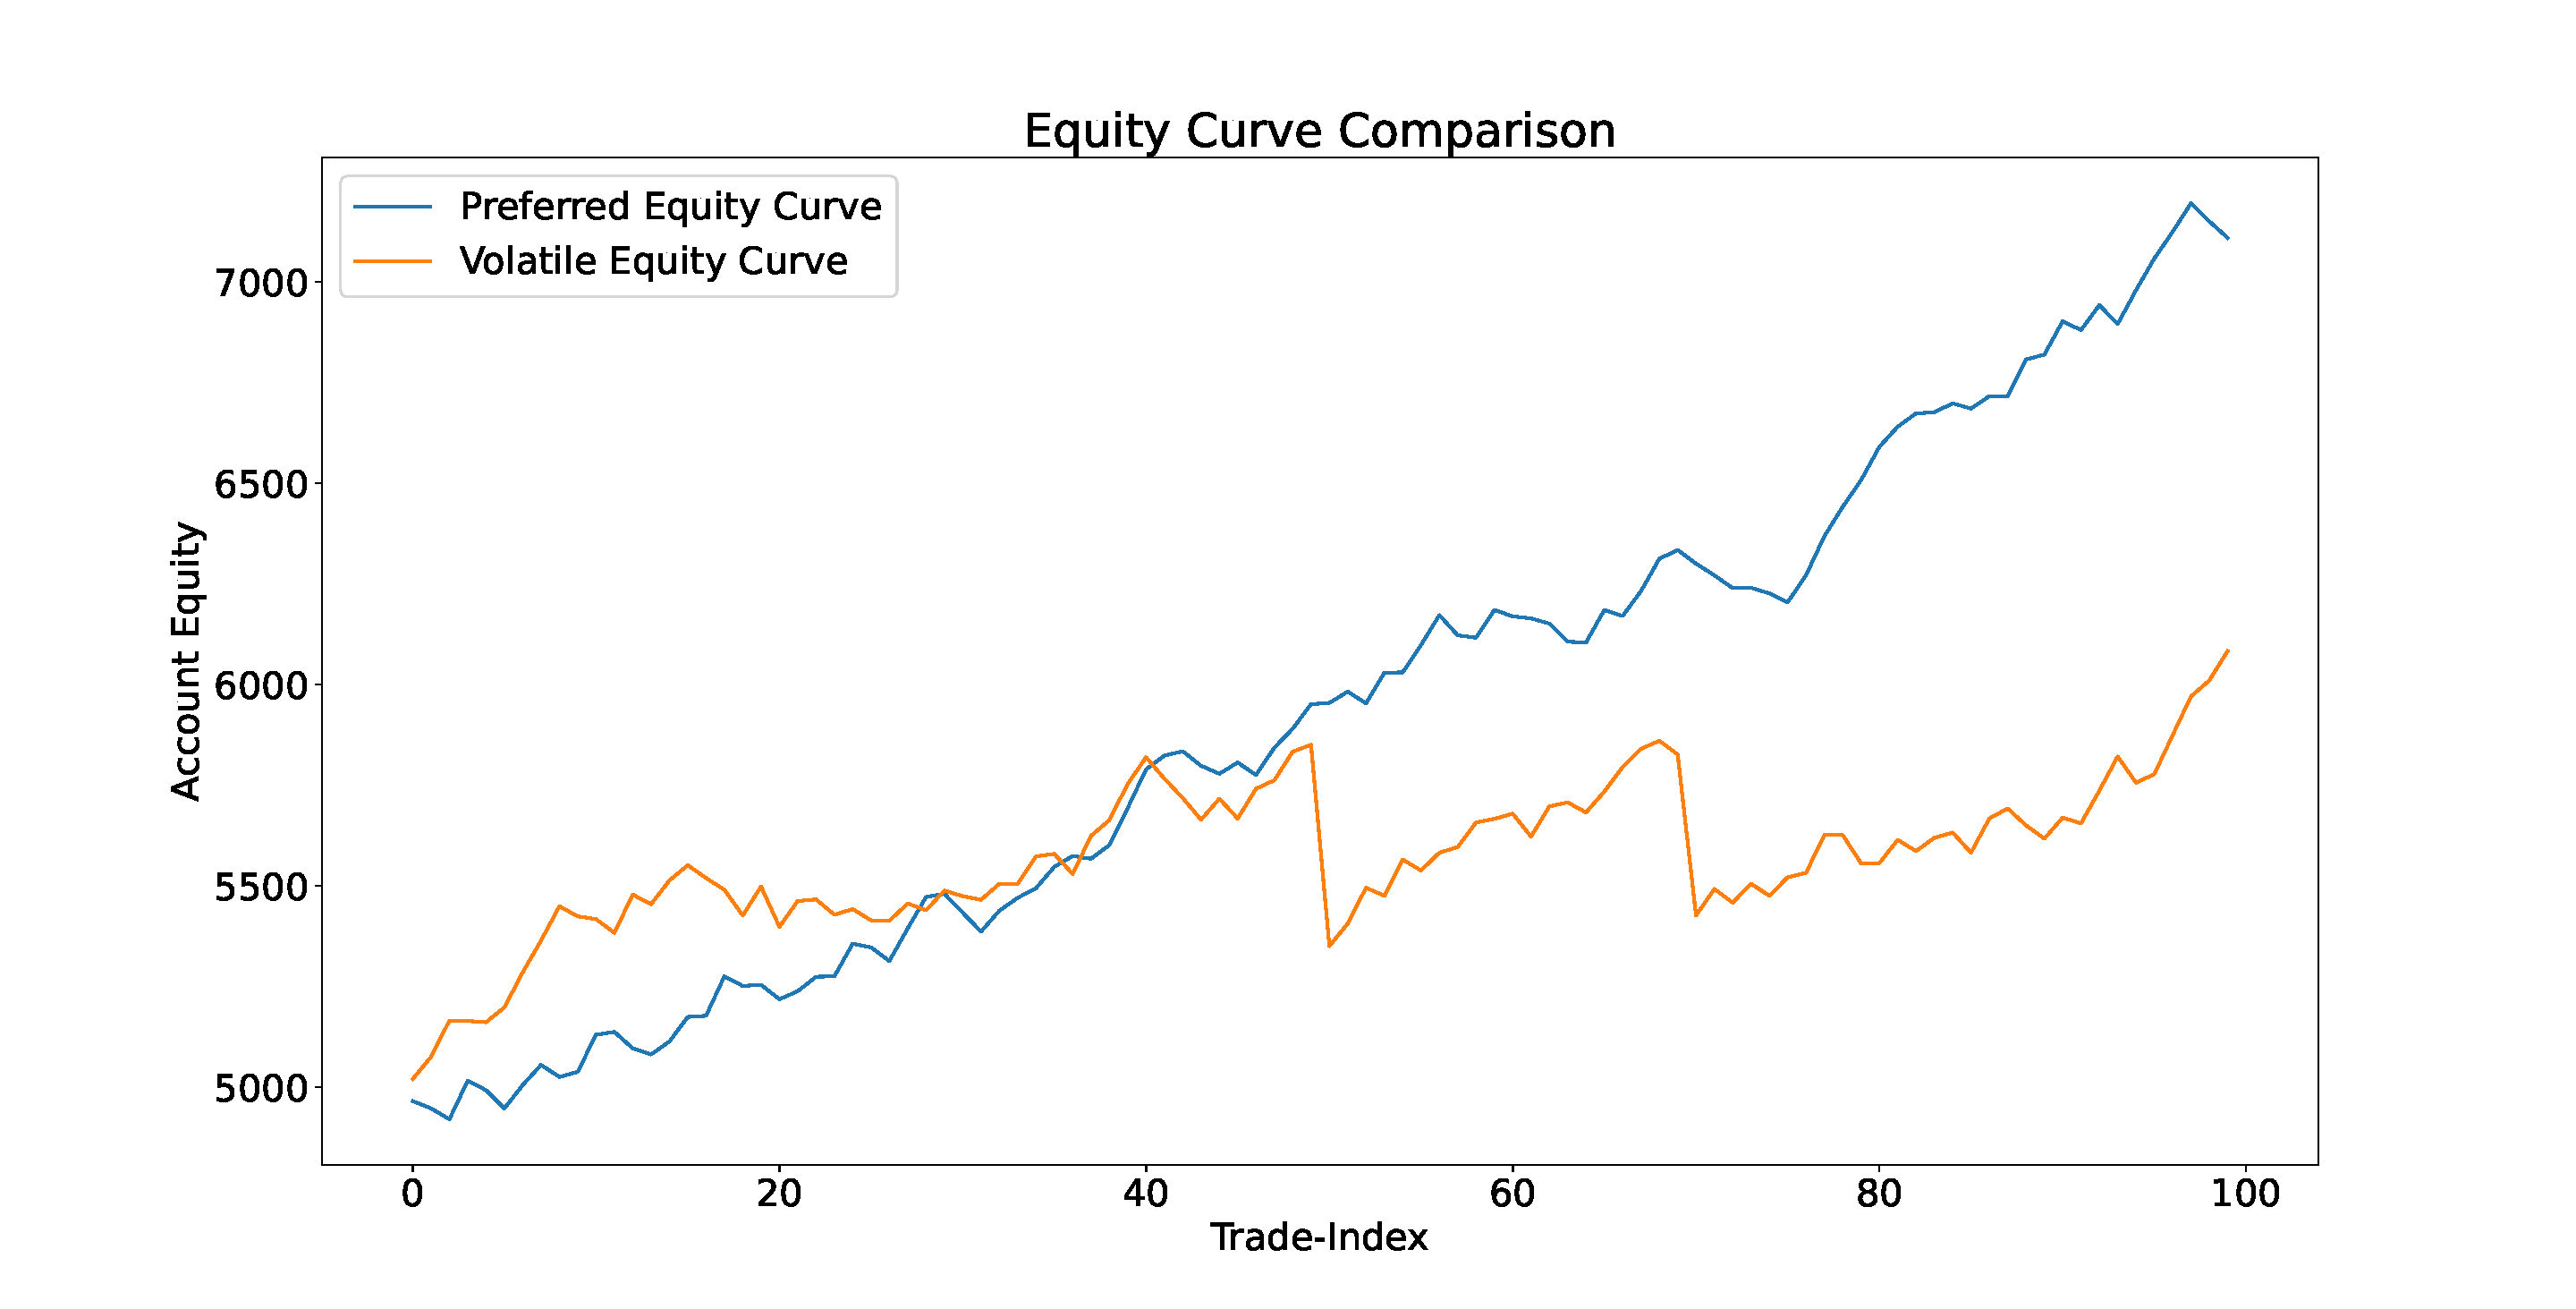
\includegraphics[width=\textwidth]{images/trading-strategies/equity-curve}
    \caption{Equity Curve Comparison}
    \label{fig:equity-curve}
\end{figure}

\subsection{Maximum Drawdown}

The maximum drawdown (MDD) measures the largest percentage loss of an investment from its highest point (peak) to its lowest point (trough) within a specific period.
It shows the maximum loss a trading strategy incurs before the investment recovers.
The MDD is an important risk measure because it highlights the potential losses in times of crisis.
A high drawdown indicates high volatility or poor risk management \cite{mdd}.

For each point in time in the equity curve, the drawdown (DD) at time $t$ can be calculated by \cite{dd}:

\[
    \text{DD}_t = \frac{\text{Equity}_t - \text{Peak Value}_{\text{Before }t}}{\text{Peak Value}_{\text{Before }t}}

\]

\noindent
The maximum drawdown is then the minimum of all drawdowns.

\autoref{fig:max-drawdown} shows the drawdown curves for both equity curves from \autoref{chap:equity-curve}.
It is noticeable that the maximum drawdown of the more volatile equity curve is much larger, indicating a less optimal trading strategy.

\begin{figure}[H]
    \centering
    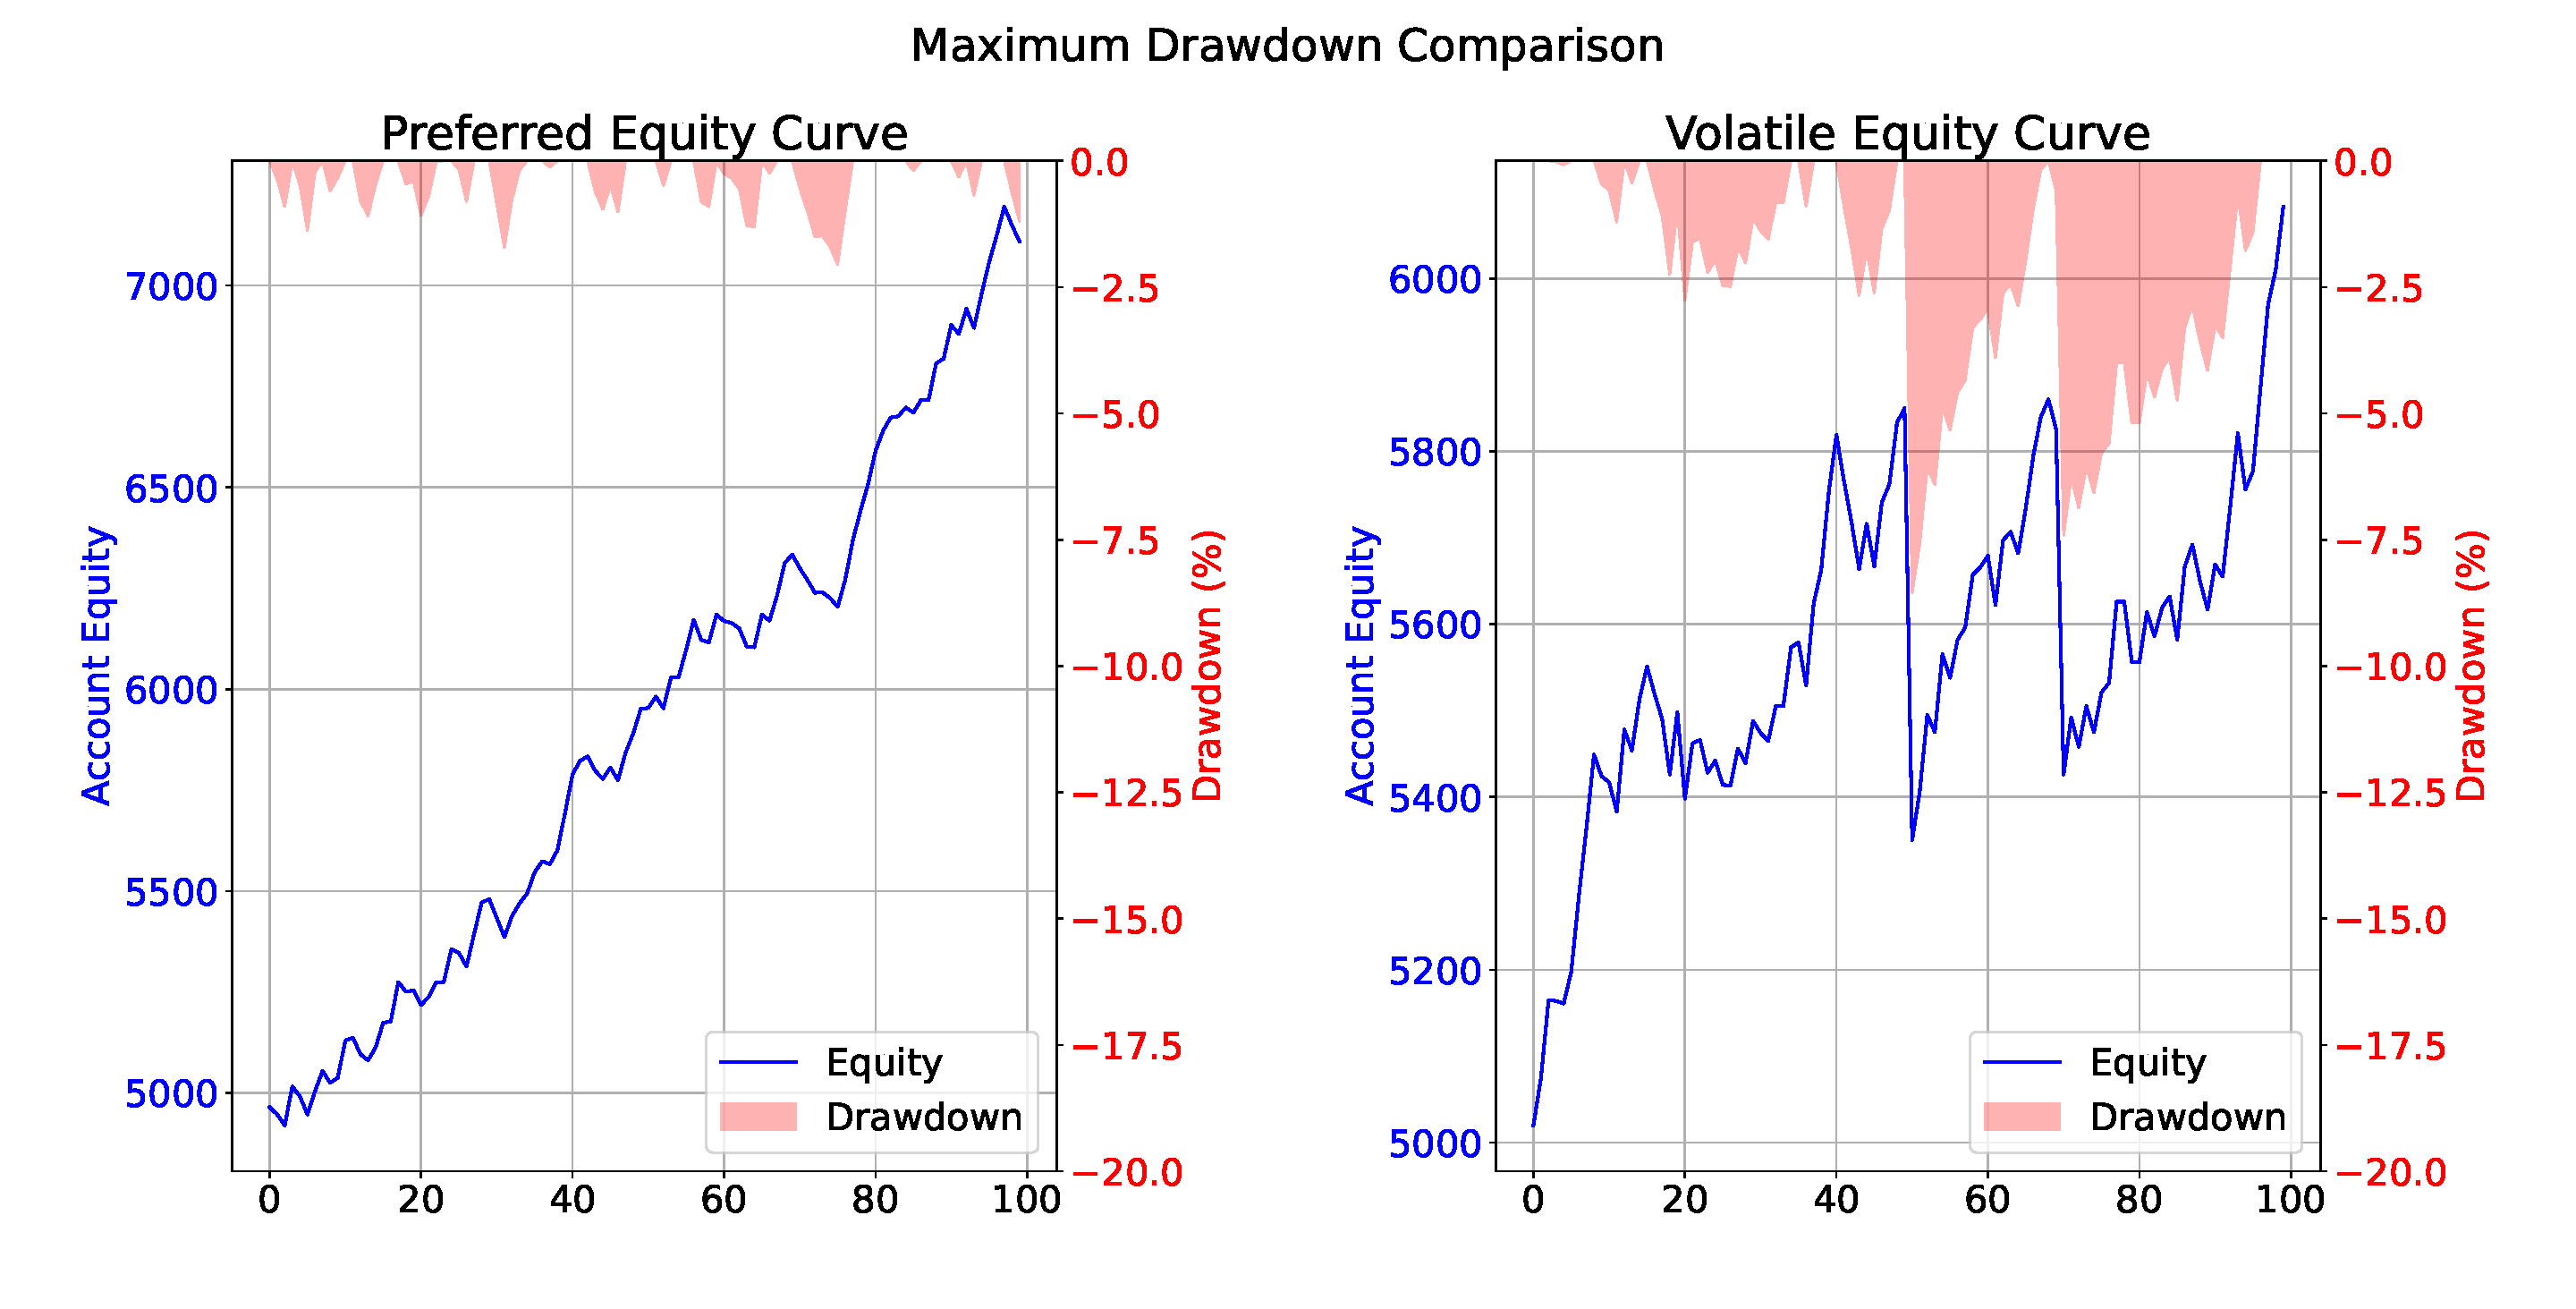
\includegraphics[width=\textwidth]{images/trading-strategies/max-drawdown}
    \caption{Drawdown Comparison}
    \label{fig:max-drawdown}
\end{figure}

\subsection{Maximum Gain and Maximum Loss}

The maximum loss indicates the largest loss within the tested period.
This metric is crucial for assessing the tail risk, i.e., the risk of extreme negative events \cite{max-loss}.
A strategy with a very high maximum loss may be profitable on average, but is potentially difficult to trade and may not be sustainable in live operations.
Especially in combination with the drawdown, the maximum loss provides an indication of the financial burden a strategy can entail.

The maximum gain describes the highest profit achieved with a single trade.
This metric allows conclusions to be drawn about the \textit{opportunity profile} of a strategy, meaning how large the potential profits can be under optimal conditions \cite{max-gain}.

However, a very high maximum gain is not necessarily positive.
In many cases, a single upward outlier is the result of random market movements and can distort overall performance.
Strategies that rely heavily on such individual results tend to be more unstable and more susceptible to market changes \cite{max-gain}.

The combination of maximum loss and maximum gain makes it possible to evaluate strategies in terms of their return-risk asymmetry.
A strategy that enables high profits but also carries a high risk of loss must be evaluated differently than a strategy with a smaller range but consistent performance.

\subsection{Standard Deviation of Profits}

The standard deviation of profits is a statistical measure that indicates how much the individual results of a trading strategy deviate from the average profit or loss per trade.
It therefore measures the volatility of individual results and allows conclusions to be drawn about the stability, consistency, and risk of a trading strategy \cite{std}.

Formally, the standard deviation of profits is defined as follows:

\[
    \sigma = \sqrt{\frac{1}{n} \sum_{i=1}^n (p_i - \bar{p})^2}
\]

\noindent
Where:

\begin{itemize}
    \item \(p_i\) is the profit (or loss) of the \(i\)th trade,
    \item \(\bar{p}\) is the average profit across all trades,
    \item \(n\) is the number of trades.
\end{itemize}

\noindent
The standard deviation is particularly valuable when comparing strategies with similar average profits.
It helps assess the consistency of performance \cite{std}:

\begin{itemize}
    \item \textbf{Low standard deviation:} Consistent results, more robust against noise and randomness.
    \item \textbf{High standard deviation:} Large fluctuations between trades, higher psychological and overfitting risks.
\end{itemize}

\noindent
A low standard deviation means that the results of individual trades are close to the average, while a high standard deviation indicates highly fluctuating results.
In particular, strategies with few but very large wins and many small losses (or vice versa) usually have a high standard deviation, which increases the risk of performance misjudgment.

\subsection{Win Rate}
\label{chap:win-rate}

Another important metric for trading strategy comparison is the win rate (or win ratio).
It is the percentage of profitable trades in relation to the total number of trades and is calculated as follows:

\[
    \text{WinRate} = \frac{\text{Number Of Winning Trades}}{\text{Total Number Of Trades}} \cdot 100
\]

\noindent
For example, if for a total of 20 trades, 16 have been profitable, the win rate is $\frac{16}{20} \cdot 100 = 80\%$.

The greatest limitation of the win rate is that a high win rate does not always indicate a profitable trading strategy \cite{win-rate}.
For example, if the win rate is 80\% with an average gain of \$20 per profitable trade and an average loss of \$90 per unprofitable trade, the weighted average is $\frac{80 \cdot 20 - (100 - 80) \cdot 90}{100} = \$-2$.
Assuming a different strategy with 40\% win rate, but with an average gain of \$70 per profitable trade and an average loss of \$15 per unprofitable trade, its weighted average is $\frac{40 \cdot 70 - (100 - 40) \cdot 15}{100} = \$19$.
The second strategy has a much lower win rate, but its long-term outcome is much higher, compared to the first one.